\documentclass[aspectratio=169]{beamer}

%% Juego de caracteres usado en el archivo fuente: UTF-8
\usepackage{ucs}
\usepackage[utf8x]{inputenc}
\uselanguage{spanish}
%Para la identación del español
\usepackage[spanish]{babel}
\usepackage{animate}
\setbeamercovered{dynamic}
\useinnertheme{rectangles}

% There are many different themes available for Beamer. A comprehensive
% list with examples is given here:
% http://deic.uab.es/~iblanes/beamer_gallery/index_by_theme.html
% You can uncomment the themes below if you would like to use a different
% one:
%\usetheme{AnnArbor}
%\usetheme{Antibes}
%\usetheme{Bergen}
%\usetheme{Berkeley}
%\usetheme{Berlin}
%\usetheme{Boadilla}
%\usetheme{boxes}
%\usetheme{CambridgeUS}
%\usetheme{Copenhagen}
%\usetheme{Darmstadt}
%\usetheme{default}
%\usetheme{Frankfurt}
%\usetheme{Goettingen}
%\usetheme{Hannover}
%\usetheme{Ilmenau}
%\usetheme{JuanLesPins}
%\usetheme{Luebeck}
\usetheme{Madrid}
%\usetheme{Malmoe}
%\usetheme{Marburg}
%\usetheme{Montpellier}
%\usetheme{PaloAlto}
%\usetheme{Pittsburgh}
%\usetheme{Rochester}
%\usetheme{Singapore}
%\usetheme{Szeged}
%\usetheme{Warsaw}

%Para la identación del español
\usepackage[spanish]{babel}

\title{Fantasy}

% A subtitle is optional and this may be deleted
%\subtitle{Optional Subtitle}

\author{Stimey}
% - Give the names in the same order as the appear in the paper.
% - Use the \inst{?} command only if the authors have different
%   affiliation.

%\institute[Escuela Superior de Ingeniería] % (optional, but mostly needed)
%{
%  \inst{1}%
%  Department of Computer Science\\
%  University of Somewhere
%  \and
%  \inst{2}%
%  Department of Theoretical Philosophy\\
%  University of Elsewhere}
% - Use the \inst command only if there are several affiliations.
% - Keep it simple, no one is interested in your street address.

\date{25 de abril de 2019}
% - Either use conference name or its abbreviation.
% - Not really informative to the audience, more for people (including
%   yourself) who are reading the slides online

%\subject{Theoretical Computer Science}
% This is only inserted into the PDF information catalog. Can be left
% out. 

% If you have a file called "university-logo-filename.xxx", where xxx
% is a graphic format that can be processed by latex or pdflatex,
% resp., then you can add a logo as follows:

% pgfdeclareimage[height=0.5cm]{university-logo}{university-logo-filename}
% \logo{\pgfuseimage{university-logo}}

% Delete this, if you do not want the table of contents to pop up at
% the beginning of each subsection:
%\AtBeginSubsection[]
%{
%  \begin{frame}<beamer>{Índice}
%    \tableofcontents[currentsection,currentsubsection]
%  \end{frame}
%}

% Let's get started
\begin{document}

\begin{frame}
  \titlepage
%  \begin{center}
%  Luis Gutiérrez Flores\\
%Nicolás Ruiz Requejo\\
%Jesús Rodríguez Heras\\
%Arantzazu Otal Alberro\\
%Alejandro Segovia Gallardo\\
%Alejandro José Caraballo García\\
%Gabriel Fernando Sánchez Reina	
%  \end{center}
  
\end{frame}

\begin{frame}{Índice}
  \tableofcontents
  % You might wish to add the option [pausesections]
\end{frame}

\section{¿Qué es fantasy?}
\begin{frame}{¿Qué es fantasy?}
\begin{block}{Fantasy}
	Aplicación web para realizar juegos educativos con la finalidad de aprender sobre un tema en particular.
\end{block}
\begin{figure}[h]
	\centering
	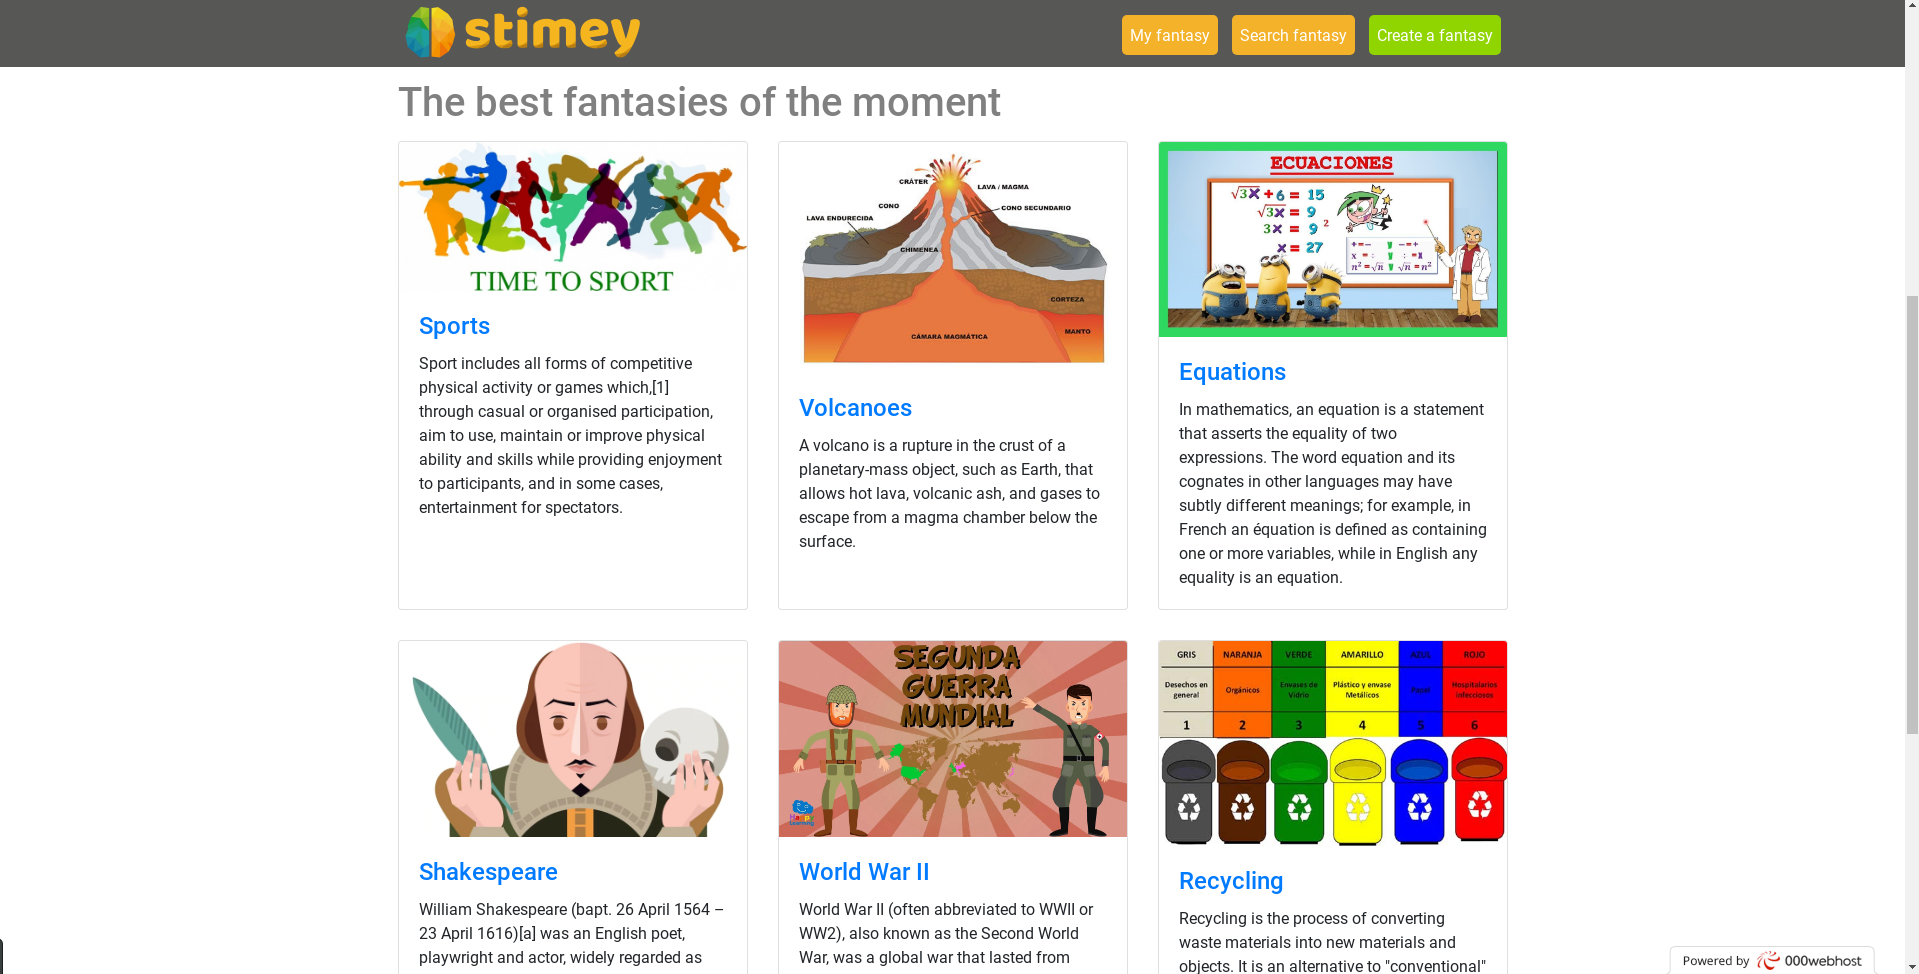
\includegraphics[scale=0.2]{Fantasy.png}
\end{figure}
\end{frame}



\section{Crear nuestra propia fantasía}
\begin{frame}{Crear nuestra propia fantasía}
Para crear nuestra propia fantasía tendremos que seguir los siguientes pasos:
\begin{itemize}
	\item Nos dirigimos a la siguiente dirección: \textcolor{red}{poner el enlace}
	\item A continuación, damos click en icono de crear una nueva fantasía (poner la fotito).
%	\begin{figure}[h]
%		\centering
%		\includegraphics[scale=0.25]{Bacground.png}
%	\end{figure}
\end{itemize}
\end{frame}

\begin{frame}{Crear nuestra propia fantasía}
\begin{itemize}
	\item Luego, nos aparecerá la siguiente pantalla (poner la fotito).
%	\begin{figure}[h]
%		\centering
%		\includegraphics[scale=0.25]{Bacground.png}
%	\end{figure}
\end{itemize}
\end{frame}

\begin{frame}{Crear nuestra propia fantasía}
\begin{itemize}
	\item Ahora, tenemos que añadir un fondo a nuestra fantasía. Para ello, haremos click en el icono de añadir un background (poner la fotito).
%	\begin{figure}[h]
%		\centering
%		\includegraphics[scale=0.25]{Bacground.png}
%	\end{figure}
	\item En la ventana emergente rellenamos los datos de la fantasía (poner la fotito con palabritas tipo prueba y tal).
%	\begin{figure}[h]
%		\centering
%		\includegraphics[scale=0.25]{Bacground.png}
%	\end{figure}
	\item Una vez rellena esta parte, le damos a ``siguiente''.
\end{itemize}
\end{frame}

\begin{frame}{Crear nuestra propia fantasía}
\begin{itemize}
	\item En esta ventana, rellenamos (los datos que sean y fotito).
%	\begin{figure}[h]
%		\centering
%		\includegraphics[scale=0.25]{Bacground.png}
%	\end{figure}
	\item Cuando hayamos terminado, pinchamos sobre ``siguiente''.
\end{itemize}
\end{frame}

\begin{frame}{Crear nuestra propia fantasía}
\begin{itemize}
	\item En esta ventana, rellenamos (los datos que sean y fotito).
%	\begin{figure}[h]
%		\centering
%		\includegraphics[scale=0.25]{Bacground.png}
%	\end{figure}
	\item Cuando hayamos finalizado con la edición de la fantasía, pinchamos sobre ``finalizar''.
\end{itemize}
\end{frame}

\begin{frame}{Crear nuestra propia fantasía}
\begin{itemize}
	\item Llegados a este punto tenemos lo siguiente (fotito de la fantasía completa).
%	\begin{figure}[h]
%		\centering
%		\includegraphics[scale=0.25]{Bacground.png}
%	\end{figure}
\end{itemize}
\end{frame}

\begin{frame}{Crear nuestra propia fantasía}
\begin{itemize}
	\item Para crear un punto activo, damos click en icono de añadir un punto activo (poner la fotito).
%	\begin{figure}[h]
%		\centering
%		\includegraphics[scale=0.25]{Bacground.png}
%	\end{figure}
	\item Para entrar en la edición del punto activo, damos doble click sobre el punto activo y se nos abrirá la siguiente ventana emergente (poner la fotito).
%	\begin{figure}[h]
%		\centering
%		\includegraphics[scale=0.25]{Bacground.png}
%	\end{figure}
\end{itemize}
\end{frame}

\begin{frame}{Crear nuestra propia fantasía}
\begin{itemize}
	\item Rellenamos el punto activo como deseemos y, una vez terminado, le damos a finalizar (poner la fotito con el punto activo relleno de pruebas).
%	\begin{figure}[h]
%		\centering
%		\includegraphics[scale=0.25]{Bacground.png}
%	\end{figure}
\end{itemize}
\end{frame}

\end{document}


